% This is samplepaper.tex, a sample chapter demonstrating the
% LLNCS macro package for Springer Computer Science proceedings;
% Version 2.20 of 2017/10/04
%
\documentclass[runningheads]{llncs}
%
\usepackage{graphicx}
\usepackage{amssymb}
\usepackage{amsmath}
\usepackage{color}
\usepackage{babel}
\usepackage{algorithm}
\usepackage{algorithmic}


% Used for displaying a sample figure. If possible, figure files should
% be included in EPS format.
%
% If you use the hyperref package, please uncomment the following line
% to display URLs in blue roman font according to Springer's eBook style:
% \renewcommand\UrlFont{\color{blue}\rmfamily}

\begin{document}
%
\title{End-Effector Exploration Drive for Effective Motor Learning}
%
%\titlerunning{Abbreviated paper title}
% If the paper title is too long for the running head, you can set
% an abbreviated paper title here
%
\author{Emmanuel Daucé\inst{1}\orcidID{0000-0001-6596-8168}}
%
\authorrunning{E. Daucé}
% First names are abbreviated in the running head.
% If there are more than two authors, 'et al.' is used.
%
\institute{Institut de Neurosciences de la Timone, CNRS/Aix-Marseille Univ, France
\email{emmanuel.dauce@univ-amu.fr}}
%
\maketitle              % typeset the header of the contribution
%
\begin{abstract}
We develop a learning framework that implements the inversion of a target distribution
of effects to train a controller. When the target distribution is uniform, this
setup implements an efficient exploration policy. The main idea is to use and maintain a simplified effect model together with the online update of the policy.
Combined with an extrinsic reward, it is shown to provide a faster 
training than traditional off-policy techniques. 
The framework is mostly devoted to the case of motor learning, when
the number of degrees of freedom is large and the final effector space
is small and bounded.   
\keywords{Intrinsic reward  \and Model-based Exploration \and Motor learning}
\end{abstract}
%
%
%
\section{Introduction}

Recent developments in artificial intelligence have produced important qualitative leaps in the field of pattern recognition (identification of objects, faces, speech recognition, ...) in video games and assisted driving. 
They have also enabled the emergence of generative models for images, video and language. The key element that explains the success of these algorithms is the extraction of statistical invariants from data, via auto-encoding mechanisms, from data sets of arbitrary dimensions. The codes are constructed during training using the gradient descent technique. After learning, they provide synthetic descriptors of the situations encountered, which are necessary and sufficient for the production of appropriate responses.  Once learned, they thus constitute very powerful generative models of the input data. Nevertheless, the learning of these invariants currently requires a considerable amount of data, real or simulated, which makes the learning algorithms dependent on the available databases, and gives the data collection (or simulation) process a disproportionate place. Furthermore, while the capabilities of these algorithms approaches (and sometimes exceeds) those of human subjects for specific tasks, they never achieve the universal skills and general adaptability of the human brain. 

Nevertheless, a number of tasks considered as simple, falling under universal competences specific to the animal world, are struggling to find a convincing artificial implementation... This is the field of action selection and motor control. For instance, a number of tasks involving the fine manipulation of objects, as well as movement in natural environments, and their combination through motor commands updated in real time according to the state of the sensors, are major challenges that are currently concentrating the efforts of the main players in the digital revolution.
Reinforcement Learning in particular remains rather limited in the field of robotic control (compared to video games). The huge developments obtained on virtual environments (from nothing) are difficult to transfer to real robotics (millions of parts/millions of tests, risk of breakage...) and simulators are expensive to develop.

The brain, on the other hand, is capable of developing motor skills in a very wide range of areas over a long developmental phase.   
The main function of the brain is to enable movement, to orientate the body and to enable it to use the environment to its own advantage. The control of an articulated body is particularly complex, and if we consider humans, it takes about a year to learn bipedal walking. The brain's ability to learn new abilities and skills is particularly striking, but it is not specific to humans. The brain in general adapts to its environment. Animals modify their behaviour flexibly according to their own history. 

%The nervous system is characterized by a high degree of noise and variability: synapses are stochastic, neurons are fatiguable, synaptic connections are plastic. Neurons taken at the individual level are extremely unreliable as a unit of information processing (to the same extent as would be biologically possible). There is an "excess" of noise in the nervous system, which leads to (i) an ability to "produce" noise/information; (ii) an ability to "sample" the response space; (iii) a principle of scan/exploration/collection (foraging) of the sensory/motor space (one does not immediately return to where one has already explored).

%Physiology
%\begin{itemize}
%	\item >80\% reciprocal connections in the cortex (Van Essen et al, 1992)
%	\item Intrinsic Activity (Fox et al, 2006)
%	\item Stochastic Behaviour (Shadlen, Newsome, 1998)
%	\item Plasticity of Hebb (Bi and Poo, 1998)	
%\end{itemize}
%Motor control
%\begin{itemize}
%	\item end-effector control  (independent of the starting point) (Graziano et al, 2002)
%	\item Spatial and temporal compositionality of motor tasks (Diedrichsen \& Kornysheva, 2015, Kadmon Harpaz et al, 2019)
%\end{itemize}


The probabilistic view to learning cause-effect relationships is at the core of many recent developments in machine learning, with a body of optimization techniques known as “variational inference” implementing model training from data \cite{kingma2013auto}. 
%One key idea is here to take inspiration from some theories developed in machine learning to reconsider the brain at the light of probabilistic inference and optimization.
%A first and not  yet fully unveiled example is how the brain learns the consequence of its own action though experiencing interactions with the world [2]. A second example in vision is how the eye selects its next saccade in order to deepen the understanding of its visual environment [3].
Taking motor control learning and action selection as a main guideline, our general objective is to decipher the respective contributions of information seeking \cite{mohamed2015variational}, learning improvement \cite{schmidhuber1991curious} and utility maximization \cite{sutton2018reinforcement} in the selection of actions in an ecological setting, with both perspectives in modelling brain function and developing innovative brain-inspired machine learning techniques for control and robotics.

\section{Method}

Formally speaking, the set of circuits, neurons that process the sensory signals and produce a motor response
is the \emph{control space} and the body, muscles and environment is the \emph{operation space}. 
The circuits and neurons are digital.
The body and environment is a continuous physical system 

There are generally two ways to design controllers.  
In analog control, both the controller and the environment are dynamical systems. 
More precisely : a controller is organised around its sensors / actuators with a measure and 
an action. The controller acts on the environment (change according to internal states). 
The environment acts on the controller (that changes according to its internal state -- memory)
The control of a dynamic system generally relies on a \emph{model}. The controller is capable to mimic the
behavior of the environment, and know the effect of its actions on the environment. When a certain objective is given, it can 
act so as to reach the objective through \emph{model inversion}.
This kind of controller needs a model, that is generally given. When no model is given, it needs both to train a model from 
the data, and train an inverse model that fits the action to the objective.
A main drawback of model inversion is the fact that, in most cases of interest (like the control of an articulated body), the models are not invertible and no single definite control can be established from a given objective. 

In contrast, in a digital (discrete) world, all you
need is to establish a one to one correspondence between stimuli and actions. For a given stimulus, you need to find the action by
matching the input with a template action. Given a set of pre-defined actions, all you have to do is just pick the one that matches the most the input.  
In order to learn how to act, the agent is guided by a reward signal (much cheaper than an exact set point).
%much easier to train from data. 
But : the rewards can be sparse.
Utility-based control defines an important quantity : the utility : the long term sum of rewards \cite{sutton2018reinforcement}.
The Reinforcement Learning agent is agnostic about what the world is. It is just acting so as to maximize the utility.
Supported by the solid principles of dynamic programming, this agent is in principle easier to train than an analog one, but
a hidden difficulty lies in finding a good training dataset for the agent. A classical problem in that case is the lack of sampling efficacy due to the closed-loop structure of the control task, where the examples encountered are statistically dependent on the controller parameters, 
providing a risk of a self referential loop and local optimum.

A main difference between the two approaches is thus the presence (or the absence) of a definite model of the external world.   Knowing the effect of our own actions in the world provides ways to anticipate and do planning to reach an objective, at the cost of maintaining and updating a model of the world. 

The opposition between model-free and model-based control has provoked many debates in the reinforcement learning community, with a preference toward model-free approaches for they are cheaper to maintain and easier to control, leaving unsolved the problem of the sampling efficacy and causing very long training sessions in moderately complex environments.
 
Our argument here is that the sampling efficacy is bound to the problem of training a model, and one can not expect to have an efficient sampling without a minimal model of the \emph{effect} of action. This model does not need to be perfectly accurate, but it needs to be good enough to allow the agent to efficiently sample its environment in order to grab all the disposable information in relation to the task at hand. We assert here that a simple \emph{effect model} is enough to provide all the needed variability in the effect of an action or a policy. 

%{\color{magenta} Our approach is different from the `curious'', and ''novelty seeking'' agents.}
%{\color{blue}
%In order to circumvent this problem, a body of work has developed curiosity and novelty-seeking in agents, independently from the utility of actions.  [REFS]
%Novelty seeking relies on building a model of the environment to which the current data is compared. A data showing inconsistencies with the model is considered as "interesting" and should attract the attention of the agent, independently of its extrinsic value.  }

We assume for simplicity that the environment is not hidden to the agent, i.e. the environment is fully observable. We also assume a discrete updating of states and actions, like in classic reinforcement learning.
Then, if $s$ is the state of the environment (or a context), and $a$ an action performed by the agent, consider $e$ as the \emph{effect} of the action performed by the agent in that particular state. The effect can be a short-term effect, like reading a new state from the environment. It can also be a long term effect, like winning or loosing a game, or reaching an objective $s^*$ in the future. Because there is a lot of uncertainty on the effect of an action, it is modeled as a probability distribution $p(E|s,a)$.
When the effect is not dependent on a context, it can be noted more simply $p(E|a)$.
Given a certain policy $\pi(a|s)$, one can also consider the average distribution of effects obtained when applying that specific policy, namely 
\begin{align}\label{eq:effect-model}
p(E|s) = \mathbb{E}_{a\sim \pi(A|s)} p(E|s,a)
\end{align}  

In goal-directed control, if $e$ is an expected effect, an \emph{inverse control policy}, whose role is to maximize the chance to reach the effect, can be defined using Bayes rule as:
\begin{align}\label{eq:inv-policy}
\pi(a|s,e) = \frac{p(e|s,a)\pi(a|s)}{p(e|s)}
\end{align}
That is said the inversion of the model in a probabilistic setup. 

Consider now a case where the objective is not to reach a certain effect, but rather to define a policy that allows to explore uniformly the range of all possible effects. Let $\pi^*$ be the policy that should provide this uniform sampling of the effect. 

Then, we can write 
\begin{align}
\pi^*(a|s) &= \mathbb{E}_{e\sim p(E|s,a)} \pi^*(a|s,e)\frac{p^*(e|s)}{p(e|s,a)}
\end{align}
with $p^*(e|s)$ the target distribution of effects (here a uniform distribution).
The right side of the equation provides an estimation of the optimal policy based on a sample $e$ of the effect of the action. Unfortunately, the optimal inverse control policy $\pi^*(a|s,e)$ is unknown. A shortcut is to approximate it with the current inverse control policy $\pi(a|s,e)$.
In that case, it happens from equation (\ref{eq:inv-policy}) that the formula simplifies to :
\begin{align}\label{eq:bayesian-update}
\pi^*(a|s) &\simeq \mathbb{E}_{e\sim p(E|s,a)} \pi(a|s,e)\frac{p^*(e|s)}{p(e|s,a)}\\
&= \pi(a|s) \mathbb{E}_{e\sim p(E|s,a)} \frac{p^*(e|s)}{p(e|s)}
\end{align}
which provides a correction term to the current policy based on a sample of its effect, in order to approach a target distribution of effects.

Consider now that the current policy $\pi$ is parameterized by a set of parameters noted $\theta$. For simplicity, we assume in the following that $\theta=(Q,\beta)$ i.e. $\forall s,a$,
\begin{align}
\pi(a|s) = \frac{\exp \beta Q(s,a)}{\sum_{a'\in \mathcal{A}} \exp \beta Q(s,a')}
\end{align}
that is the softmax policy parameterized by an action-value function $Q$ and an inverse temperature $\beta$.

Then, noting $Z= \sum_{a'\in \mathcal{A}} \exp \beta Q(s,a')$, 
\begin{align}
\log \pi(a|s) = \beta Q(s,a) - \log Z
\end{align}

From equation (\ref{eq:bayesian-update}), it comes:
\begin{align}
 Q(s,a) - Q^*(s,a) &\simeq \frac{1}{\beta} \left(\log \mathbb{E}_{e\sim p(E|s,a)} \frac{p(e|s)}{p^*(e|s)} + \log Z - \log Z^*\right)\\
 &\leq \frac{1}{\beta}  \left(\mathbb{E}_{e\sim p(E|s,a)} [\log p(e|s) - \log p^*(e|s)] + \log Z - \log Z^*\right) \label{eq:TD-err}
\end{align}
making it possible to define an upper bound on the \emph{error} on $Q(s,a)$ from the sampling of its effect.

Assuming that the effect model $p(e|s)$ is known makes it possible to update $Q(s,a)$ with the last effect sample $e$ like:
\begin{align}\label{eq:Q-update}
Q(s,a) \leftarrow & Q(s,a) - \alpha (\log p(e|s) - \log p^*(e|s))
\end{align}  
This update is only a fraction of the total error, but renders the current policy closer to the optimal one. A side effect of this update is that it also changes the effect model that includes the contribution of the policy (see eq. (\ref{eq:effect-model})). Repeating the operation with a small $\alpha$ and different samples of $a$ and $e$ should, on average, reduce the divergence between $\pi$ and $\pi^*$.


\subsection*{Link with reinforcement learning}
Equation (\ref{eq:Q-update}) also provides an interesting identity when considering the classical (reward-based) TD-error. If we assume now ($i$) that $Q^*$ is the parameter of an optimal policy according to the extrinsic rewards provided by the environment, and ($ii$) that $e$ is a future trajectory over states and actions, then, by construction, 
\begin{align}\label{eq:Q-RL}
Q^*(s,a) - Q(s,a) &= \mathbb{E}_{e\sim p^(E|s,a)} R(e) - Q(s,a)\nonumber \\
			      &=\mathbb{E}_{e\sim p^(E|s,a)}\sum_{(s',a')\in e} r(s',a') - Q(s,a) \nonumber\\
                  &\simeq  \mathbb{E}_{e\sim p(E|s,a)}  \frac{1}{\beta} [\log p^*(e|s) - \log p(e|s) + C]
\end{align}
then, up to a constant, the sum of the future rewards is consistent with the log-probability of a future effect. The higher the reward, the more probable the effect (here a trajectory over future states), showing that more rewarding trajectories are visited more often under the (softmax)-optimal policy.   
Conversely, when a supervised prior $p^*(e|s)$ is provided and the current effect model is known, it is possible to provide a corresponding ``reward'' $R(e)$, i.e.
\begin{align}
\mathbb{E}_{e\sim p^(E|s,a)} R(e) \cong Q(s,a) + \frac{1}{\beta} \mathbb{E}_{e\sim p^(E|s,a)}[\log p^*(e|s) - \log p(e|s)] 
\end{align}
making it possible, for instance, to provide an intrinsic reward that implements a uniform prior on effects, knowing a baseline policy (for instance a uniform policy) and the corresponding baseline distribution of effects (that is not necessary uniform!).

\subsection*{Link with variational inference}
Assume now that the extrinsic rewards provided by the environment are not consistent with the intrinsic drive defined by the target distribution of effects $p^*(e|s)$. This correspond to the case where two objectives are followed, namely both maximizing the future rewards and explore in a uniform way the space of the possible effects. From formula (\ref{eq:Q-RL}), the target action-value of $\hat{Q}$ is:
\begin{align}
\hat{Q}(s,a) \equiv \mathbb{E}_{e\sim p^(E|s,a)} R(e) - \frac{1}{\beta} (\log p^*(e|s) - \log p(e|s))
\end{align}
And, after reading $e$, the update of $Q$ should look like :
\begin{align}
Q(s,a) \leftarrow (1-\alpha) Q(s,a) + \alpha  (R(e) - \frac{1}{\beta} (\log p^*(e|s) - \log p(e|s)))
\end{align}
and the TD-error should now be defined as:
\begin{align}\label{eq:var-RL}
\text{TD}(s,a,e) = Q(s,a) - R(e) + \frac{1}{\beta} (\log p^*(e|s) - \log p(e|s)))
\end{align}

Interestingly, the minimization of the error through the update of $Q$ is consistent with a variational approach to reinforcement learning, such as the ones that are developed by, e.g. \cite{levine2013guided}.
Assume $a$ being observed from sampling on the policy, then $\beta Q(s,a)\equiv \log \pi(a|s)$ is interpreted as the expected likelihood (from the model) and $R(e)$ is an observation of the actual likelihood of $a$ (such as it is provided by the environment). Here the effect $e$ is seen as the ``cause'' of the observation, that explains $R(e)$. This reversed interpretation of the causes and the effects allows to update the policy from the effect it has produced, in a reversed causal order, in accordance with the general anticausal direction of learning.

The actions difference of this approach, w.r.t. the model-free approaches used in the literature \cite{toussaint2009robot,levine2013guided}, is the use of a coarse \emph{model} of the effect of action. This model needs to be updated jointly with the policy, for the changing of the policy directly modifies the probability of reaching a final state. The effect model is thus expected to be coarse and simple, and may, for instance, only monitor the final state in an episodic reinforcement learning setup. 

Interestingly, in formula (\ref{eq:var-RL}), the reward $R(e)$ has the role of a regularizer with regards to the current Q-value. The sum of the future rewards can be estimated using the classical Bellman recurrence equation, i.e. $Q(s,a) \sim r(s,a) + Q(s', a')$, in which case the training procedure needs to maintain an estimate of a standard action-value function $Q_\text{ref}(s,a)$ to update the actual parameters of the policy $Q(s,a)$.  

Last, a precision hyperparameter $\lambda$ is considered to account for the different magnitudes of rewards, and manipulate the balance between reward seeking and exploration-seeking drives. The final formula used in simulations is:
   \begin{align}\label{eq:var-RL-lambda}
   \text{TD}(s,a,e) = \lambda(Q(s,a) - R(e)) + \frac{1}{\beta} (\log p^*(e|s) - \log p(e|s)))
   \end{align}


\section{Results}

We present in simulation a pilot implementation of the principle presented in the previous section. The principal idea is to illustrate an important feature of biological motor control, that is the control of an effector showing many degrees of freedom, like e.g. an articulated limb with many joints. 
In classical reinforcement learning, the action spaces are generally considered smaller than the sensory space. This is for instance the case when training a model on vintage Atari games, where the control is limited to a set of action keys \cite{mnih2013playing}.

Let $\mathcal{A}$ a set of composed actions, each possible action owning $n$ degrees of freedom, with $\mathbf{a_{1:n}} \in \mathcal{A} = {a_1,...,a_n}$. The effect space is expected to be much smaller, like it is the case in end-effector control, where only the final set point of a movement in the peripheral space is considered as the result of the action. Each degree of freedom is supposed to be independent, i.e. the choice of $a_i$ does not depend on the choice of $a_j$, so that $\pi(a_{1:n}|s) = \pi(a_1|s) \times ... \times \pi(a_n|s)$. When a single context is considered, the policy writes simply $\pi(a_{1:n})$.
The size of the action space is thus combinatorially high, and one can not expect to enumerate every possible action in reasonable computational time. 

In contrast, the effect space is bounded, and the number of all final states can be enumerated. However, the environment is constructed in such a way that some final states are very unlikely to be reached under a uniform sampling of the action space.


The first environment we consider is a grid world with only 18 states and two rooms, with a single transition allowing to pass from room A to room B (see figure \ref{fig:grid1}). Starting in the upper left corner of room A, the agent samples a trajectory $a_{1:7} \in \mathcal{A}$ from a policy $\pi$, that trajectory being composed of 7 elementary displacements (E,S,W,N). The agent does not have the capability to read the intermediate states it is passing through, it can only read the final state after the full trajectory is realized. 
    
In such an environment, a baseline uniform exploration does not provide a uniform distribution of the final states. In particular, when acting at random, the chance to end-up in the first room is significantly higher than the chance to end up in the second room.  
    
The agent starts from scratch, and has two build a policy $\pi(a)$ and an effect model $p(s)$, with $s$ the final state. 
There are two task at hand. A first task is a simple exploration task and the objective is to uniformly sample the effect space, which should imply a non-uniform sampling policy. A second task consists in reaching the lower-right corner, the state that shows the lowest probability with a uniform sampling. For that, a reward of 1 is given when the agent reaches the lower corner, and 0 otherwise.

\begin{figure}[t]\label{fig:grid1}
\centerline{
	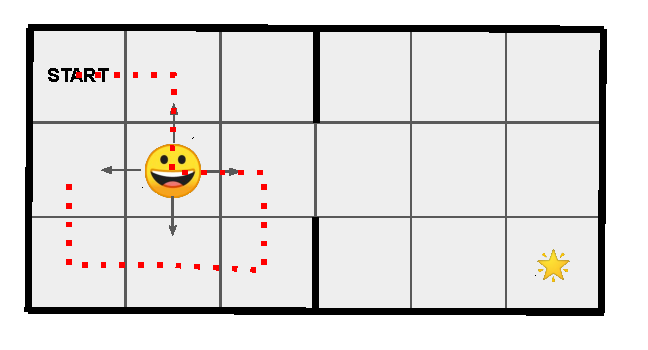
\includegraphics[width = .7 \linewidth]{../figures/env-1.pdf} 
}
\caption{A simple two-rooms environment. Starting from the upper-left corner, the agent is asked to plan a full sequence made of 7 elementary actions $a_1,...,a_7$, each elementary action being in (E,S,W,N). The only read-out from the environment is the final state, and a reward, that is equal to 1 if the final state is the lower-right corner, and 0 otherwise.}
\end{figure}

The update procedure is made of a simple loop (see algorithm \ref{algo:E3D}). The update is done online at each trial. Both the policy and the effect model are updated, with different training parameters. The general idea is to train the effect model a little more ``slowly'' than the policy, for the policy improvement to firmly take place before they are passed on the effect model. 

Stemming from a uniform policy, the effect of the E3D drive is to render the "rare" states more
attractive, for they are bound with a positive intrinsic reward, while the more commonly visited 
 states are bound with a negative reward, that reflects a form of "boredom". Marking a rare state as ``attractive'' tends to increase the number of visits, and finally lower the initial positive reward. In the case of a ``gradient'' in the likelihood of the final states, with a number of final visits inversely proportional to the distance to the initial state, the E3D drive favors a progressive ``expansion'' of the visiting territory, for each peripheral state attained will increase the probability to reach its further neighbors, up to the final limit of the state space. In small environment like the one proposed here, the limit is rapidly attained and a rapid alternance of visits is observed over the full state space. 

The final distribution of states is compared in figure \ref{fig:explore} in the case of a uniform policy and the E3D drive. In that specific setup, a strong bias in favor of the first room is observed, and a gradient of likelihood is observed from the initial state toward the lower right corner (figure \ref{fig:explore}A). In contrast, a time consistent uniform pattern of visit is observed in the second case, that illustrates the capability of the E3D drive to set up specific polices devoted to the wide exploration of the environment.     

\begin{algorithm}[t]
	\caption{End-Effector Exploration Drive (E3D)}\label{algo:E3D}
	\begin{algorithmic}
		\REQUIRE{$\alpha$, $\beta$, $\lambda$, $\eta$}
		%\STATE predict $z \sim \rho$
		\STATE $p \leftarrow$ Uniform
		\STATE $p^* \leftarrow$ Uniform
		\WHILE{number of trials not exceeded}
			\STATE sample $a_{1:n} \sim \pi(A_{1:n})$ 
			\STATE read $s,r$
			\STATE $p \leftarrow (1-\eta) p + \eta \mathbf{1}_{S=s} $ 
			\FOR{$i \in 1..n$}
			    \STATE $Q(a_i) \leftarrow (1-\alpha\lambda) Q(a_i) + \alpha\lambda r - \frac{\alpha}{\beta} (\log p(s)-\log p^*(s))$ 
			\ENDFOR
		\ENDWHILE
	\end{algorithmic}
\end{algorithm}

When a reward $r$ is provided by the environment, the question comes whether to balance the policy update procedure in favor of seeking for rewards or seeking for novel effects. By construction, the exploration drive is insensitive to the value of $\beta$, for the update is exactly proportional to $\frac{1}{\beta}$.  A high $\beta$ is associate with a small update and vice versa. this is not the case for the leftmost part of the update (equation \ref{eq:var-RL-lambda}). A high $beta$ render the agent more sensitive to the extrinsic rewards. In practice, while no reward (or a uniform reward) is provided by the environment, the agent is only guided by the exploration drive. Once a reward is encountered, it tends to overtake the initial uniform exploration, providing a firm tendency toward a reward-effective selection of action. This is in contrast with the standard epsilon-greedy strategy, imposing to balance the exploration/exploitation trade-off by hand.

The E3D approach finally provides an Online/on-Policy training procedure that conforms to the main requirements of efficient reinforcement learning, showing both an efficient exploration policy when the rewards are sparse, and the capability to monitor the exploration/exploitation tradeoff with the inverse temperature $\beta$ in function of the magnitude of the rewards.

The cumulative rewards obtained with the E3D update and a state-of-the art off-policy/epsilon greedy update are compared in figure \ref{fig:compare}, with $varepsilon$ set to 0.1. If both techniques manage to reach a reward-efficient policy in the long run, the exploration strategy developed in E3D makes it easier to reach the rewarding state, providing the reward earlier in time and developing a fast-paced reward-seeking strategy that overtakes the baseline approaches.    

\begin{figure}[t!]\label{fig:explore}
	\centerline{\bf (A)}
	\centerline{
		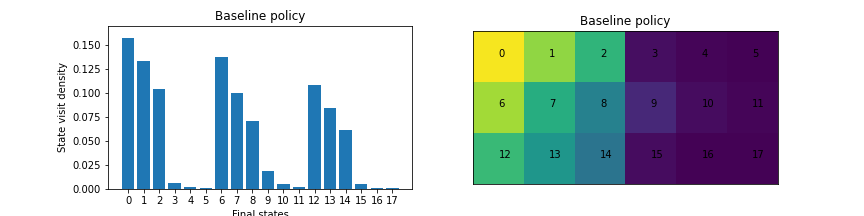
\includegraphics[width = .9\linewidth]{../figures/botteneck-baseline.png} 		
	}
	\centerline{\bf (B)}
	\centerline{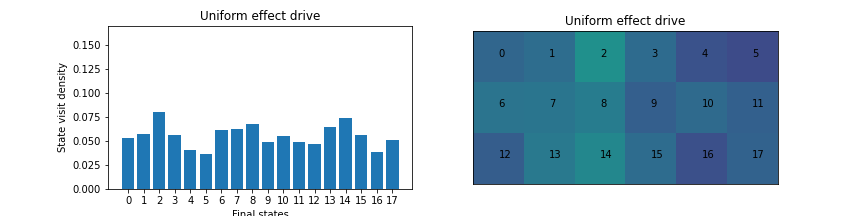
\includegraphics[width = .9\linewidth]{../figures/botteneck-uniform-drive.png} }
	\caption{Task 1 : no reward is provided by the environment. Empirical distribution of the final states, after 5000 trials. {\bf A.} Uniform policy. {\bf B.} End-Effector Exploration Drive algorithm. $\alpha=0.1$, $\beta = 1$, $\lambda=0.1$, $\eta=10^{-2}$.}
\end{figure}

\begin{figure}[t!]\label{fig:compare}

	\centerline{
		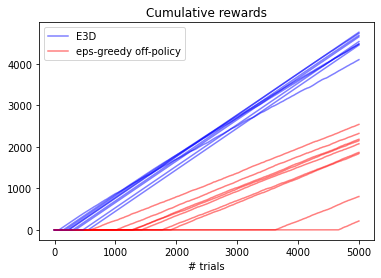
\includegraphics[width = .7\linewidth]{../figures/training-comparison.png} 		
	}
	\caption{Task 2 : a reward $r=1$ is provided by the environment when the agent reaches the lower-right corner. Cumulative sum of rewards over 5000 trials. The E3D algorithm is compared with . $\alpha=0.1$, $\beta = 100$, $\lambda=0.1$, $\eta=10^{-2}$, $\varepsilon=0.1$.}
\end{figure}

\section{Conclusions}

Despite its simplicity, our pilot training setup allows to illustrate the main features expected from the inversion of a target distribution of affects, that is the capability to rapidly explore the environment through a reciprocal update of the policy and the effect model. We found in practice that the update of the model needs to be a bit slower than that of the policy to allow for the policy to improve over time and increase the extent of the effect space in a step by step manner. By balancing the effect of the rewards with the inverse temperature parameter, it is possible to catch and exploit very sparse rewards in large environments. 

The model is developed here as a first draft in an ``end-effector'' setup, with very little influence of the context or the states visited in the monitoring of the policy. Extensions toward closed-loop state-action policies is not far from reach, for equation (\ref{eq:var-RL}) allows to exploit the Bellman recurrence to guide the exploration-driven policy with a reference action-value function, that should be updated in parallel to the model and the current policy. Extensions toward continuous action spaces are also needed in order to address effective motor control learning, which resorts to a deeper interpretation of our approach toward the variational inference setup. 
%
% ---- Bibliography ----
%
% BibTeX users should specify bibliography style 'splncs04'.
% References will then be sorted and formatted in the correct style.
%
\bibliographystyle{splncs04}
\bibliography{biblio}
%

\end{document}
